\chapter{Introducción específica} % Main chapter title

\label{Chapter2}

%----------------------------------------------------------------------------------------
%	SECTION 1
%----------------------------------------------------------------------------------------
Todos los capítulos deben comenzar con un breve párrafo introductorio que indique cuál es el contenido que se encontrará al leerlo.  La redacción sobre el contenido de la memoria debe hacerse en presente y todo lo referido al proyecto en pasado, siempre de modo impersonal.

\section{Componentes principales de hardware}
\label{sec:ejemplo}

\subsection{STM32 NUCLEO-L432KC}
La placa STM32 Nucleo-32 que se muestra en la figura \ref{fig:nucleol432kc} proporciona una forma asequible y flexible para que los usuarios prueben nuevos conceptos y construyan prototipos eligiendo entre las diversas combinaciones de funciones de rendimiento y consumo de energía que proporciona el microcontrolador STM32\citep{NUCLEOL432KC}.
\\Características:
\begin{itemize}
	\item Microcontrolador STM32L4KC en paquete 32 de pines.
	\item 1 led de usuario.
	\item 1 pulsador de reset.
	\item Conector de expansión Arduino Nano V3.
	\item Conector USB Micro-AB para ST-LINK.
	\item Opciones flexibles de fuente de alimentación.
	\item Depurador/Programador ST-LINK integrado.
	\item Compatibilidad con una amplia variedad de entornos de desarrollo integrado.
	\item Oscilador de cristal de 24MHz
	\item Compatible con Arm Mbed Enabled  
\end{itemize}
\begin{figure}[htbp]
	\centering
	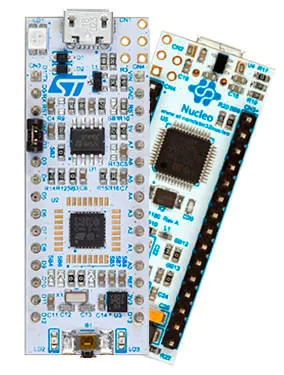
\includegraphics[width=.4\textwidth]{./Figures/nucleo-l432kc.jpg}
	\caption{Placa NUCLEO-L432KC.}
	\label{fig:nucleol432kc}
\end{figure}
\vspace{5cm}

\subsection{Módulo Comunicación LTE IOT 2 CLICK}
\label{subsec:ejemplo}
LTE IoT 2 Click es un Click board que permite la conexión a las redes LTE, con el módulo Quectel BG96 LTE , que ofrece dos tecnologías LTE destinadas a la comunicación Máquina a Máquina (M2M) e Internet de las Cosas. Este módulo es una solución de comunicación IoT integrada que admite las tecnologías LTE Cat M1 y NB1, y ofrece una alternativa a soluciones similares de red de área amplia de baja potencia (LPWAN).
LTE IoT 2 click está equipado con el módulo BG96 LTE de Quectel Wireless Solutions , que admite tecnologías LTE CAT M1 y NB1, desarrolladas con aplicaciones IoT en mente. Además, admite EGPRS a 850/900/1800/1900 MHz, lo que significa que se puede usar globalmente; no está restringido a ninguna región. El soporte para las tecnologías CAT M1 y NB1 y el consumo de energía ultra bajo hacen de este módulo una elección perfecta para la próxima tecnología 3GPP IoT.
\\Características:
\begin{itemize}
	\item Protocolos de internet integrados(TCP/UDP/PPP).
	\item Conectores SMA integrados .
	\item Leds de alimentación e indicación de estado.
	\item Conector USB para conectarlo con la aplicación de software de quectel.
	\item Interfaz UART para  intercambiar comandos. 
	\item Voltaje de alimentación 5V o 3.3V.

\end{itemize}


\begin{figure}[htbp]
	\centering
	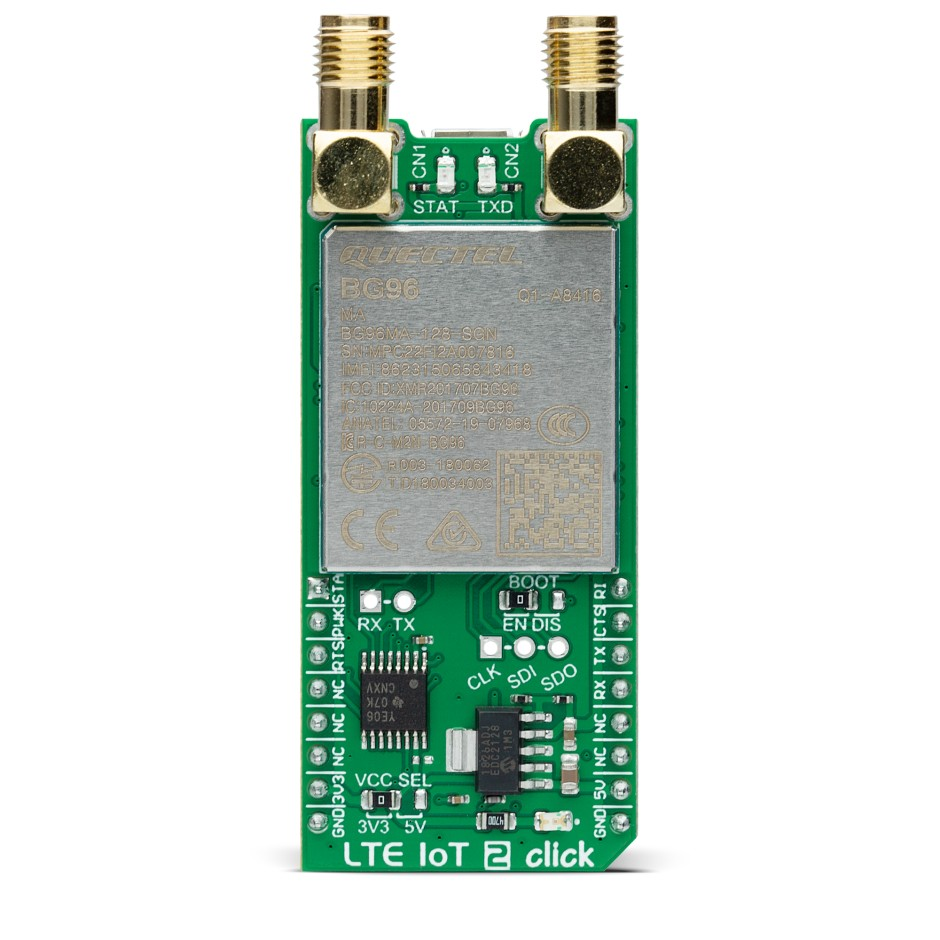
\includegraphics[width=.4\textwidth]{./Figures/moduloBG96.jpg}
	\caption{Modulo LTE IOT 2 CLICK.}
	\label{fig:modulo LTE IOT}
\end{figure}

\subsection{Sensor AHT10}
AHT10 es un sensor que permite obtener lecturas de temperatura y humedad, es de bajo costo y excelente rendimiento. El sensor es muy versátil, puede sustituir a los sensores DHT11, SHT20 y AM2302, debido a su estabilidad en entornos más hostiles. Utiliza este sensor en aplicaciones de control automático de temperatura, aire acondicionado, estaciones meteorológicas, aplicaciones en el hogar, regulador de humedad y temperatura.
\begin{figure}[htbp]
	\centering
	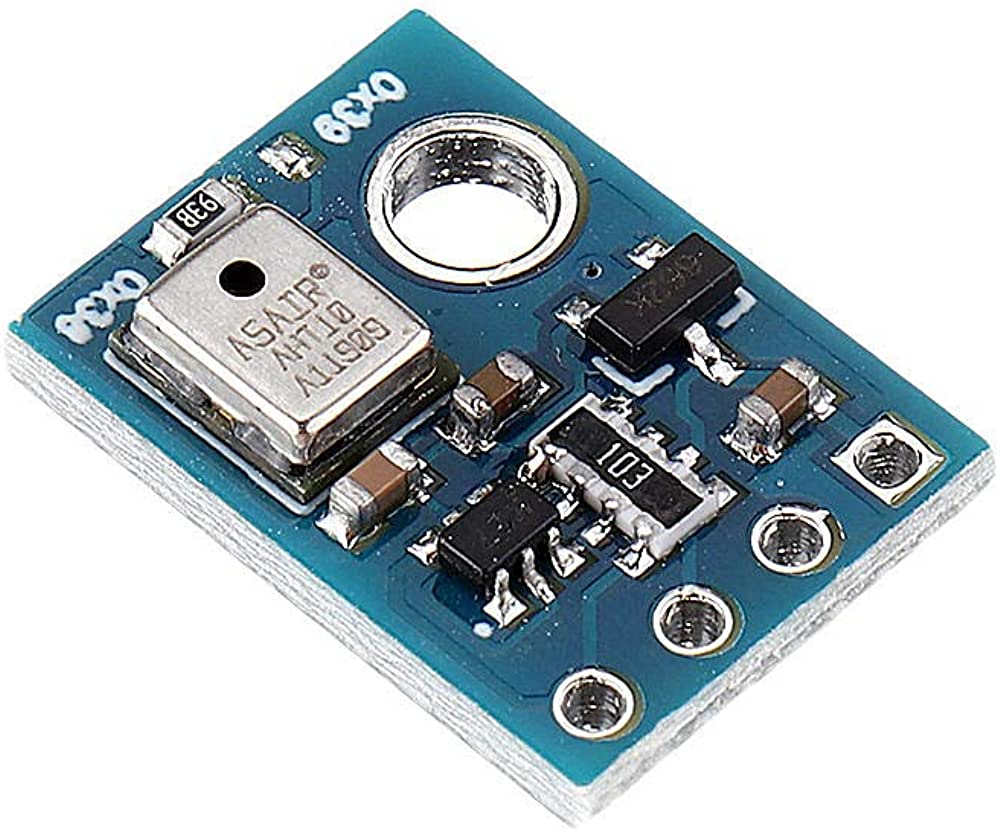
\includegraphics[width=.4\textwidth]{./Figures/aht10.jpg}
	\caption{Modulo LTE IOT 2 CLICK.}
\end{figure}

\subsection{Sensor ML8511}

El módulo ML8511 es un sensor de luz ultravioleta (UV), entrega una señal de voltaje analógica que depende de la cantidad de luz UV que detecta. Sensor ideal para proyectos de monitoreo de condiciones ambientales como el índice UV, Aplicaciones Meteorológicas, cuidado de la piel, medición industrial de nivel UV.
El sensor ML8511 detecta luz con una longitud de onda entre 280-390 nm, este rango cubre tanto al espectro UV-B como al UV-A. La salida analógica está relacionada linealmente con la intensidad UV (mW/cm2). Esta señal analógica puede ser conectada a un microcontrolador para ser convertido por un ADC y así trabajar con la medición. 
\begin{figure}[htbp]
	\centering
	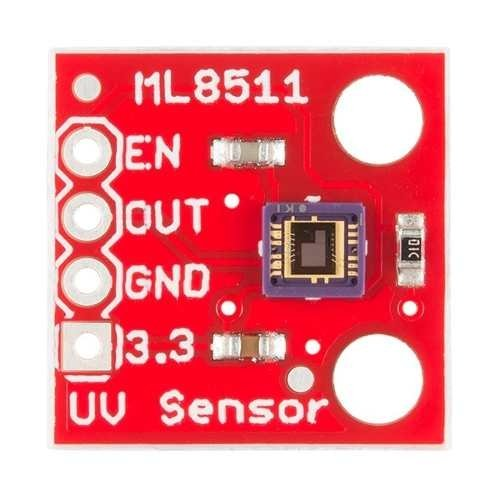
\includegraphics[width=.4\textwidth]{./Figures/ml8511.jpg}
	\caption{Modulo LTE IOT 2 CLICK.}
\end{figure}
\subsection{Sensor de Humedad de Suelo HL-69 (Resistivo)}
El módulo HL-69, un sensor de humedad de suelo resulta ser otro módulo que utiliza la conductividad entre dos terminales para determinar ciertos parámetros relacionados a agua, líquidos y humedad.
\begin{figure}[htbp]
	\centering
	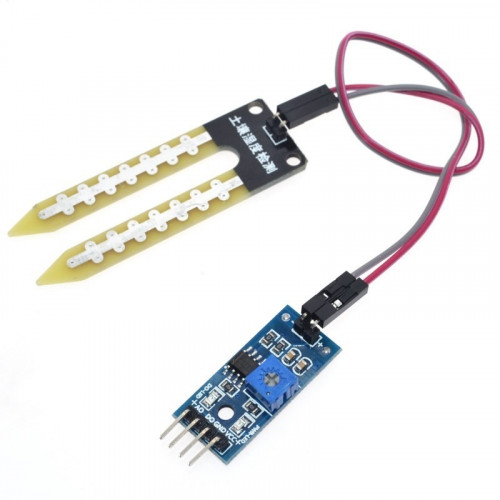
\includegraphics[width=.4\textwidth]{./Figures/sensordehumedad.jpg}
	\caption{Modulo LTE IOT 2 CLICK.}
\end{figure}

\section{Herramientas de software y testing utilizados}
\subsection{STM CUBEIDE}
STM32CubeIDE es una herramienta de desarrollo multi-OS todo en uno, que forma parte del ecosistema de software STM32Cube.STM32CubeIDE es una plataforma de desarrollo C/C++ avanzada con funciones de configuración de periféricos, generación de código, compilación de código y depuración para microcontroladores y microprocesadores STM32. Se basa en el marco Eclipse  y la cadena de herramientas GCC para el desarrollo y GDB para la depuración. Permite la integración de los cientos de plugins existentes que completan las funcionalidades del IDE de Eclipse .

STM32CubeIDE integra las funcionalidades de configuración y creación de proyectos de STM32 de STM32CubeMX para ofrecer una experiencia de herramienta todo en uno y ahorrar tiempo de instalación y desarrollo.

\subsection{FreeRTOS}
\label{subsec:FreeRTOS}
FreeRTOS es un sistema operativo en tiempo real (RTOS) líder en el mercado para microcontroladores y pequeños microprocesadores. Distribuido libremente bajo la licencia de código abierto del MIT, FreeRTOS incluye un núcleo y un conjunto creciente de bibliotecas adecuadas para su uso en todos los sectores de la industria.
FreeRTOS está diseñado con énfasis en la confiabilidad, la accesibilidad y la facilidad de uso.
\begin{figure}[htbp]
	\centering
	
\includegraphics[width=0.6\textwidth]{./Figures/logo_FreeRTOS.jpg}
	\caption{Logo FreeRTOS.}
	\label{fig:FreeRTOS}
\end{figure}
\subsection{CEEDLING}
eedling es un sistema de compilación para proyectos C que es algo así como una extensión del sistema de compilación Rake (make-ish) de Ruby. Ceedling está dirigido principalmente al desarrollo basado en pruebas en C y está diseñado para reunir CMock, Unity y CException, otros tres increíbles proyectos de código abierto sin los que no puede vivir si está creando maravillas en el lenguaje C. Con el fin de difundir la genialidad, Ceedling es un artilugio extensible con un buen mecanismo de complemento.

Ceedling es nuestra última pieza asombrosa diseñada para reunir todas nuestras ventajas para desarrolladores de C en algo más cohesivo.
\section{Protocolos de Comunicación}
\subsection{UART}
UART (universal asynchronous receiver / transmitter, por sus siglas en inglés) define un protocolo o un conjunto de normas para el intercambio de datos en serie entre dos dispositivos. UART es sumamente simple y utiliza solo dos hilos entre el transmisor y el receptor para transmitir y recibir en ambas direcciones. Ambos extremos tienen una conexión a masa. La comunicación en UART puede ser simplex(los datos se envían en una sola dirección), semidúplex(cada extremo se comunica, pero solo uno al mismo tiempo), o dúplex completo(ambos extremos pueden transmitir simultáneamente). En UART, los datos se transmiten en forma de tramas.
\subsection{I2C}
El bus de comunicaciones I2C  es un protocolo que se efectúa por medio de dos hilos. A través de estos dos hilos pueden conectarse diferentes dispositivos donde algunos de ellos serán maestros en cuanto muchos otros dispositivos serán esclavos.
\subsection{MQTT}
MQTT es un protocolo de mensajería estándar de OASIS para Internet de las cosas (IoT). Está diseñado como un transporte de mensajería de publicación/suscripción extremadamente liviano que es ideal para conectar dispositivos remotos con un espacio de código pequeño y un ancho de banda de red mínimo. MQTT hoy en día se utiliza en una amplia variedad de industrias, como la automotriz, la manufactura, las telecomunicaciones, el petróleo y el gas, etc.

\begin{figure}[htbp]
	\centering
	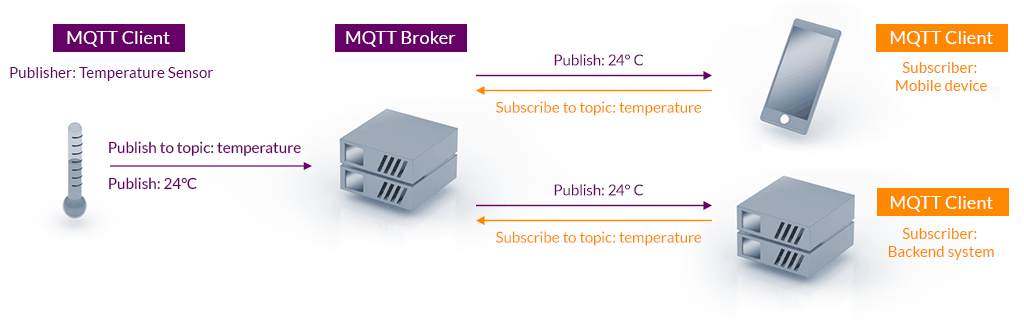
\includegraphics[width=1\textwidth]{./Figures/mqtt-publish-subscribe.png}
	\caption{Arquitectura de publicación/suscripción de MQTT.}
\end{figure}
\section{Plataformas IoT}
\subsection{Ubidots}
Ubidots una plataforma de IoT (Internet de las cosas) que habilita la toma de decisiones a empresas de integración de sistemas a nivel global. Este producto permite enviar datos de sensores a la nube, configurar tableros y alertas, conectarse con otras plataformas, usar herramientas de analítica y arrojar mapas de datos en tiempo real.
Ubidots es una plataforma en la nube para el Internet de las Cosas (IoT) que ofrece todas las herramientas necesarias que permite a las empresas desplegar soluciones IoT, ahorrarse mucho tiempo y dinero a la hora de salir al mercado y poder tomar mejores decisiones basadas en datos.En la figura se muestra un ejemplo una interfaz gráfica en ubidots.
\begin{figure}[htbp]
	\centering
	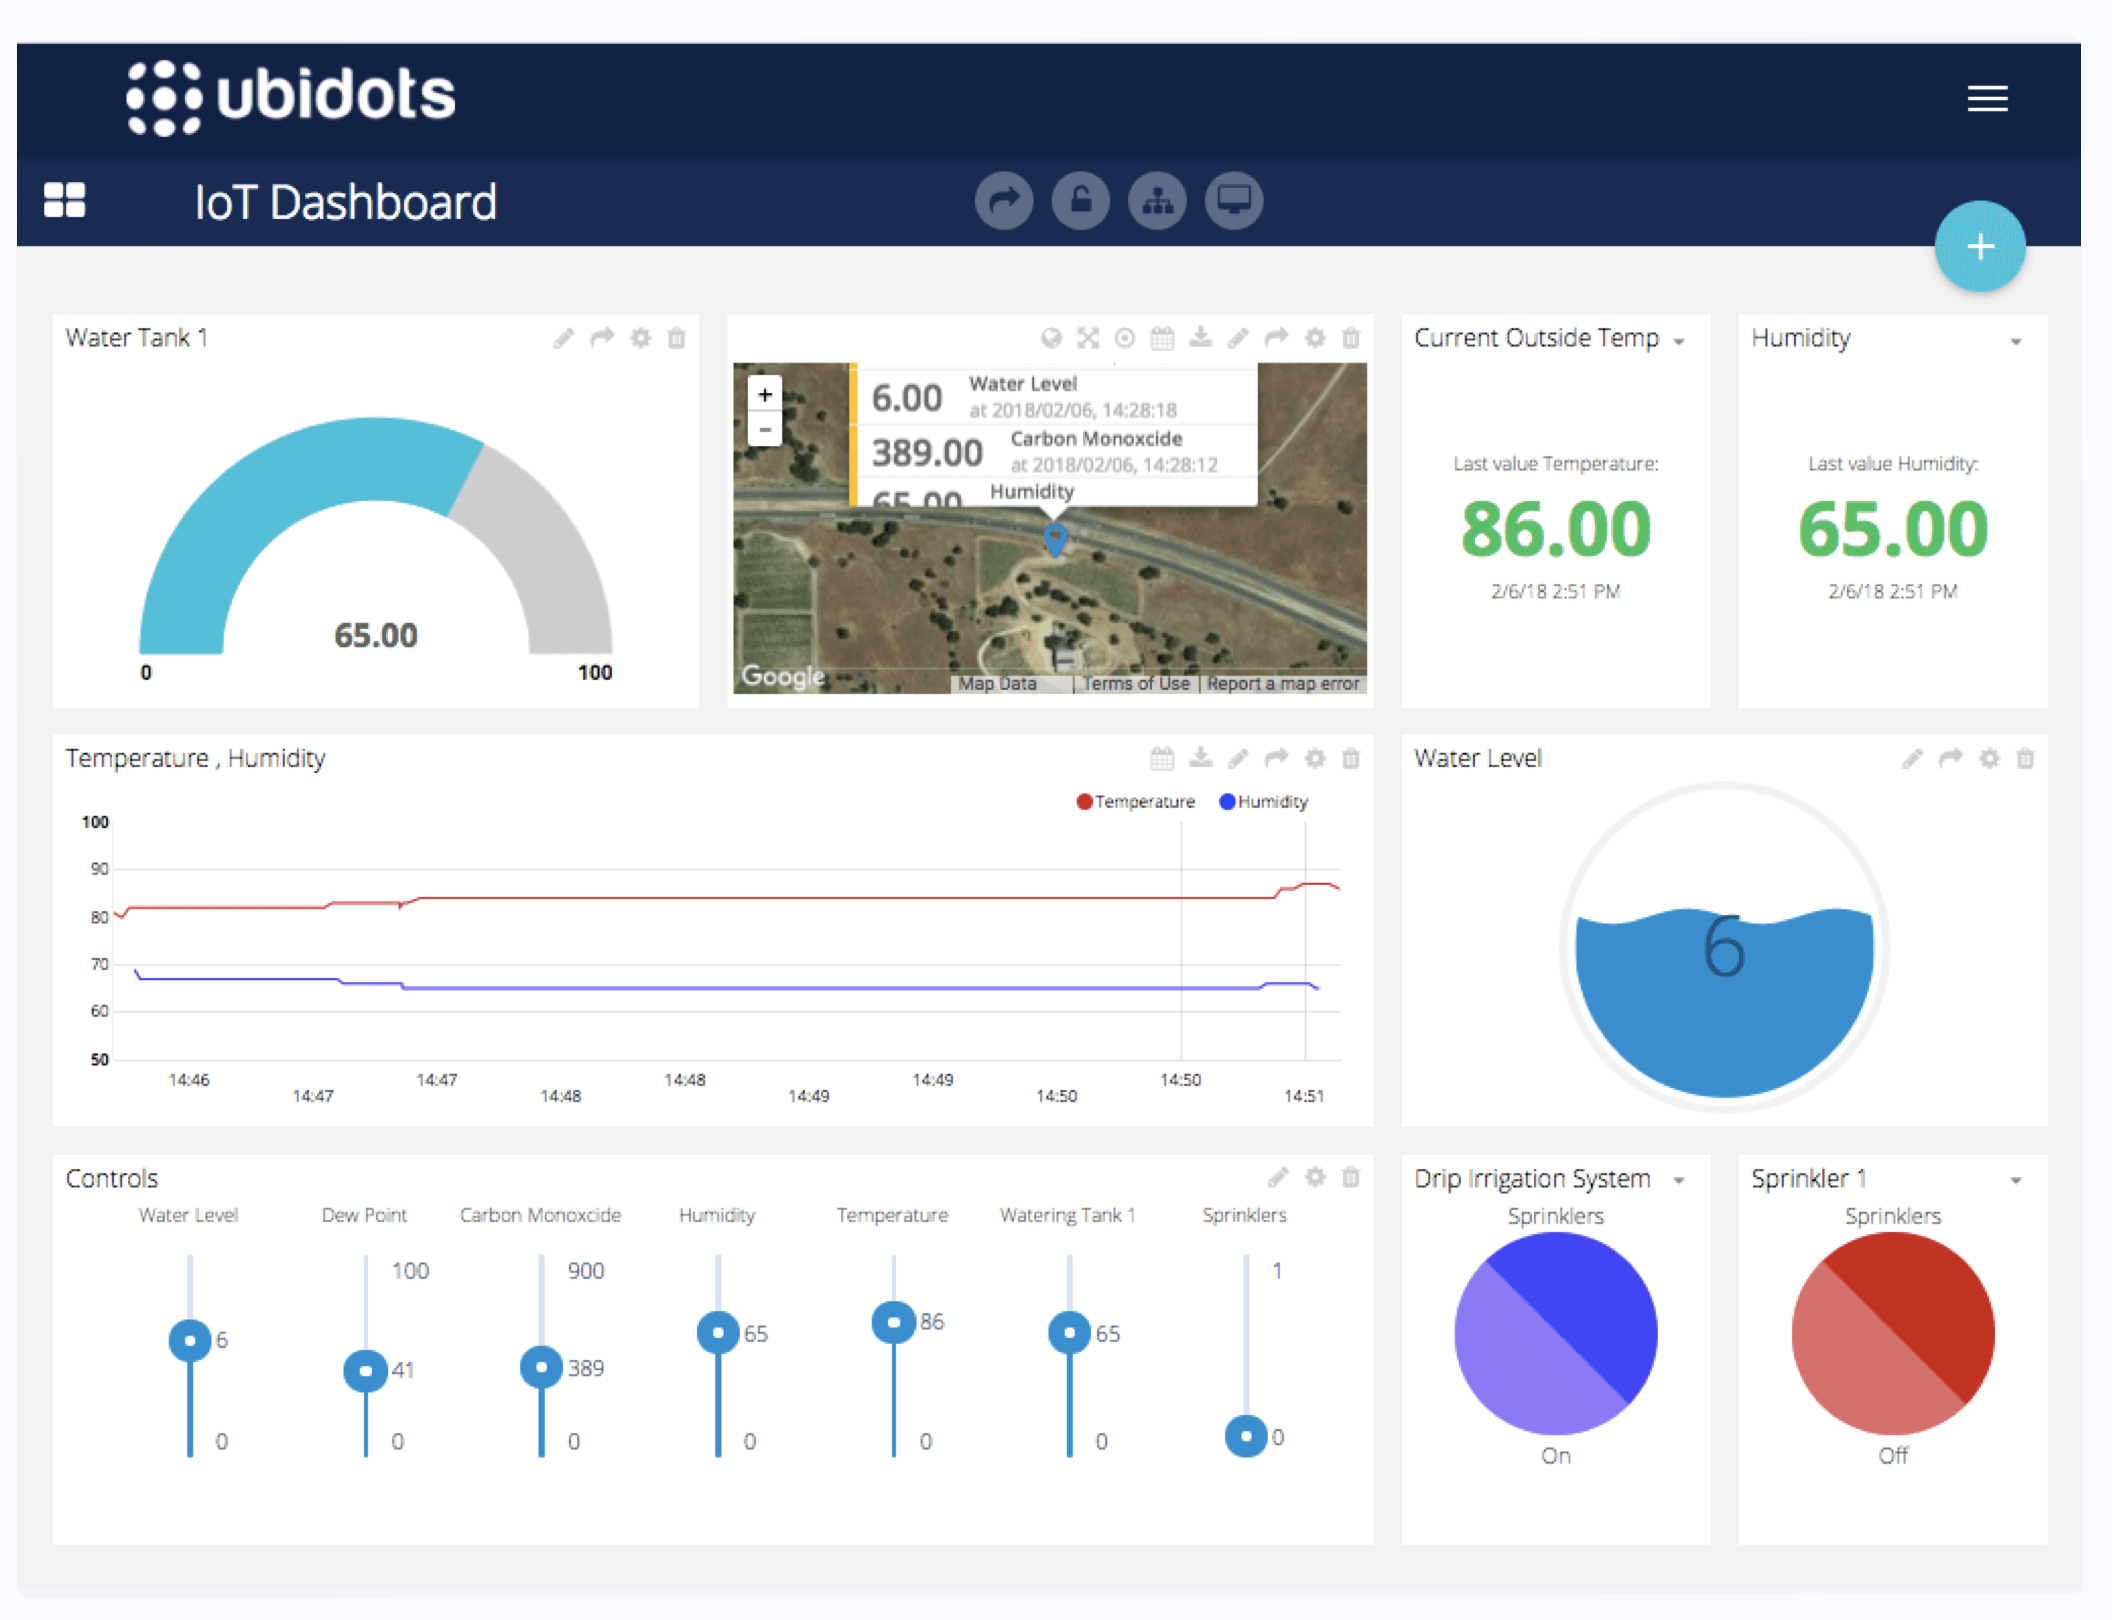
\includegraphics[width=0.6\textwidth]{./Figures/ubidots.png}
	\caption{Ejemplo Interfaz Gráfica Ubidots.}
\end{figure}
\subsection{ThingsBoard}
ThingsBoard es una plataforma IoT de código abierto para la recopilación, el procesamiento, la visualización y la gestión de dispositivos de datos.
Permite la conectividad de dispositivos a través de protocolos IoT estándar de la industria: MQTT, CoAP y HTTP, y admite implementaciones en la nube y locales. ThingsBoard combina escalabilidad, tolerancia a fallas y rendimiento para que nunca pierda sus datos.
\begin{figure}[htbp]
	\centering
	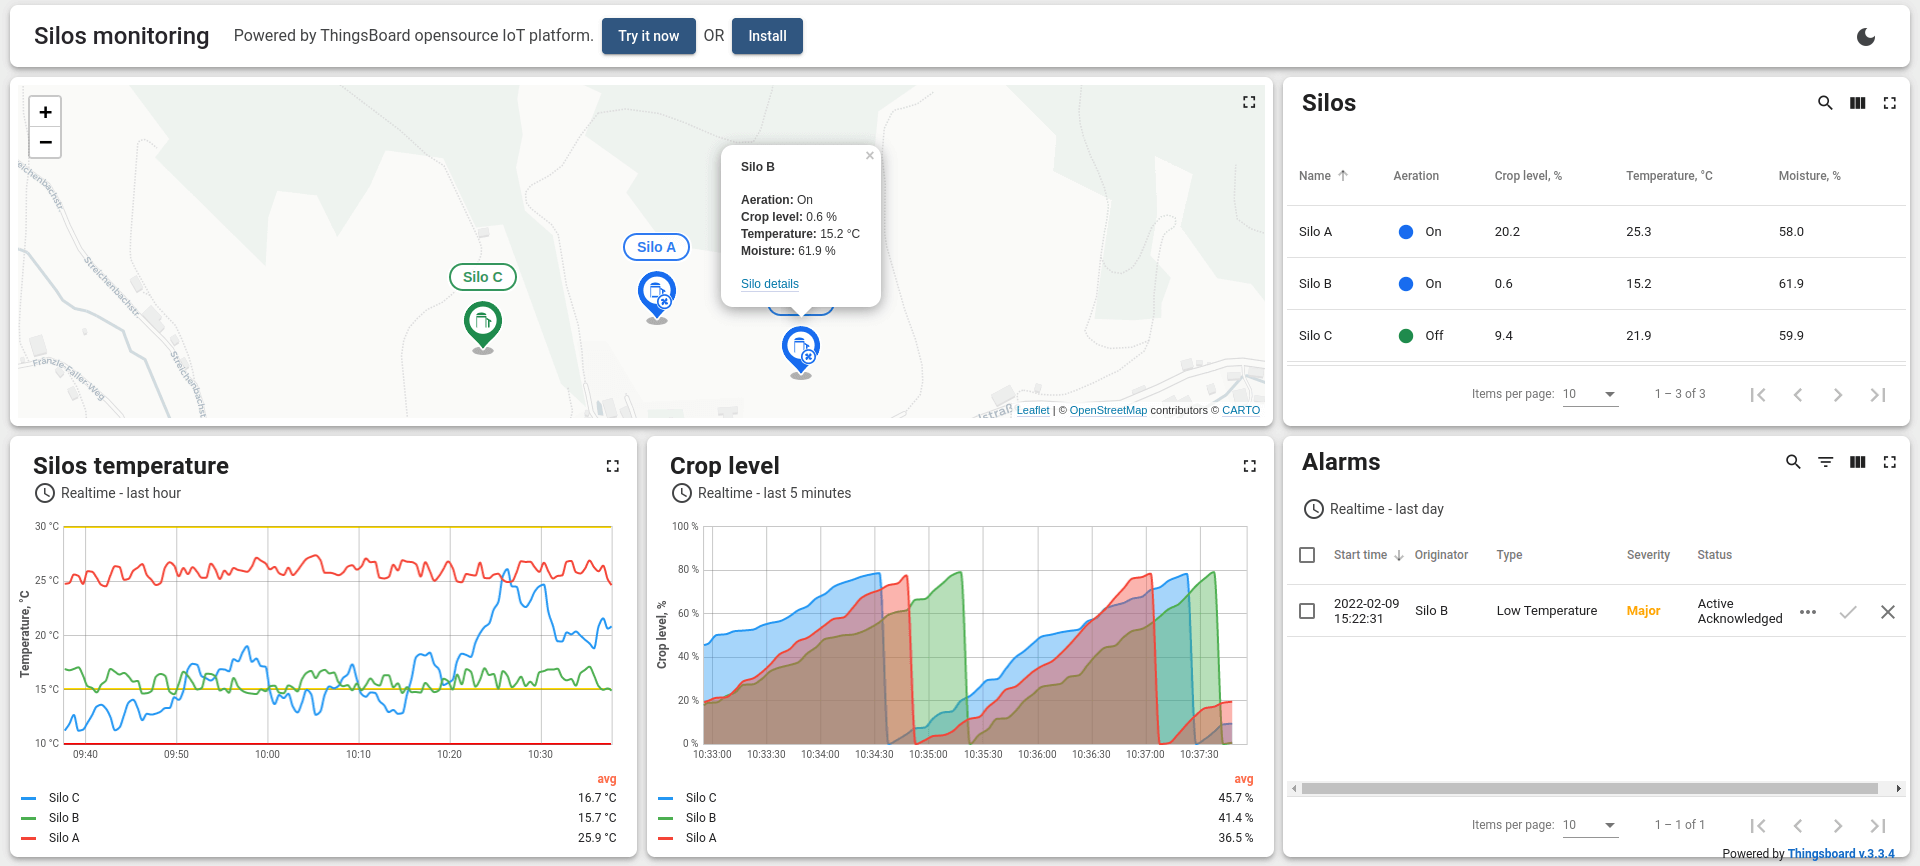
\includegraphics[width=0.8\textwidth]{./Figures/thingsboard.png}
	\caption{Ejemplo Interfaz Gráfica ThingsBoard.}
\end{figure}